\section{Multi-Leader репликация: векторные версии, объединение версий. Разрешение конфликтов при чтении и записи, параллельное разрешение конфликтов, изменение состава кластера.}

\begin{definition}
  Векторные версии
\end{definition}
\begin{itemize}
  \item Храним на каждой реплике key-value базу данных.
  \item На каждой реплике для каждой записи "ключ-значение" храним вектор
  версий.
  \item k-ая компонента вектора показывает, сколько обновлений этого ключа мы видели с реплики $k$.
\end{itemize}
\begin{definition}
  Векторные версии: обновление локальной компоненты
\end{definition}
\begin{itemize}
  \item При каждом запросе на изменение увеличиваем локальную компоненту вектора на 1 (Отличие от векторных часов в том, что там увеличивали при каждой посылке/приеме сообщения).
  \item Считается любой запрос на изменение данных, например CAS, Inc и т.д.
\end{itemize}
\begin{figure}[h]
    \centering
    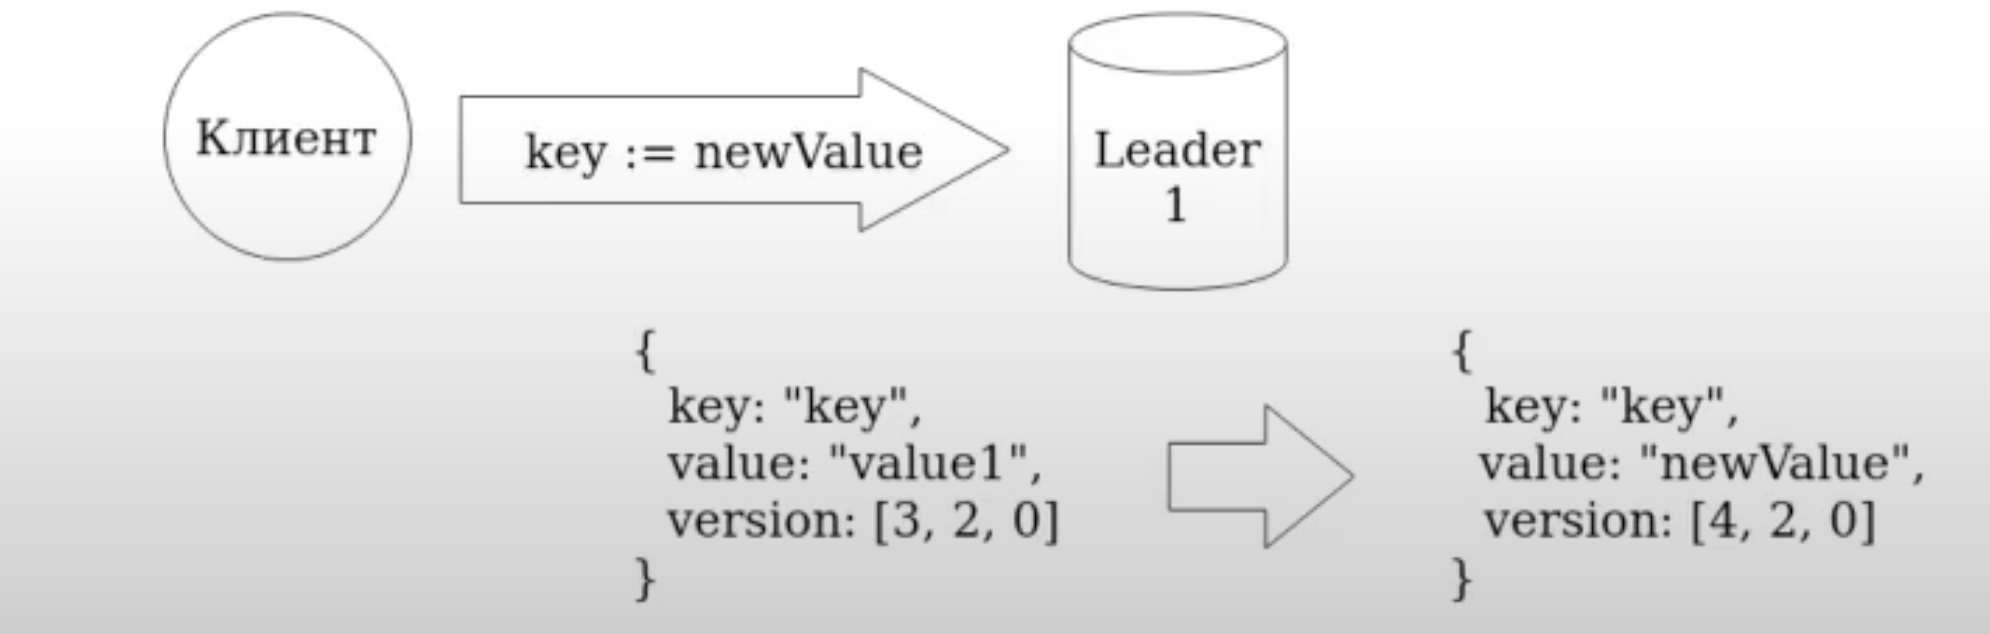
\includegraphics[scale = 0.5]{../assets/1.png}
    \caption{}
\end{figure}
\begin{definition}
  Удаление устаревших значений
\end{definition}
\begin{itemize}
  \item Реплики обмениваются локальными значениями вместе с версиями.
  \item Если $A$ happens-before $B$, то может быть $A$ удалено.
  \item $A$ happens-before $B$ - мажорирование вектора $B$ над вектором $A$.
\end{itemize}
\begin{figure}[h]
    \centering
    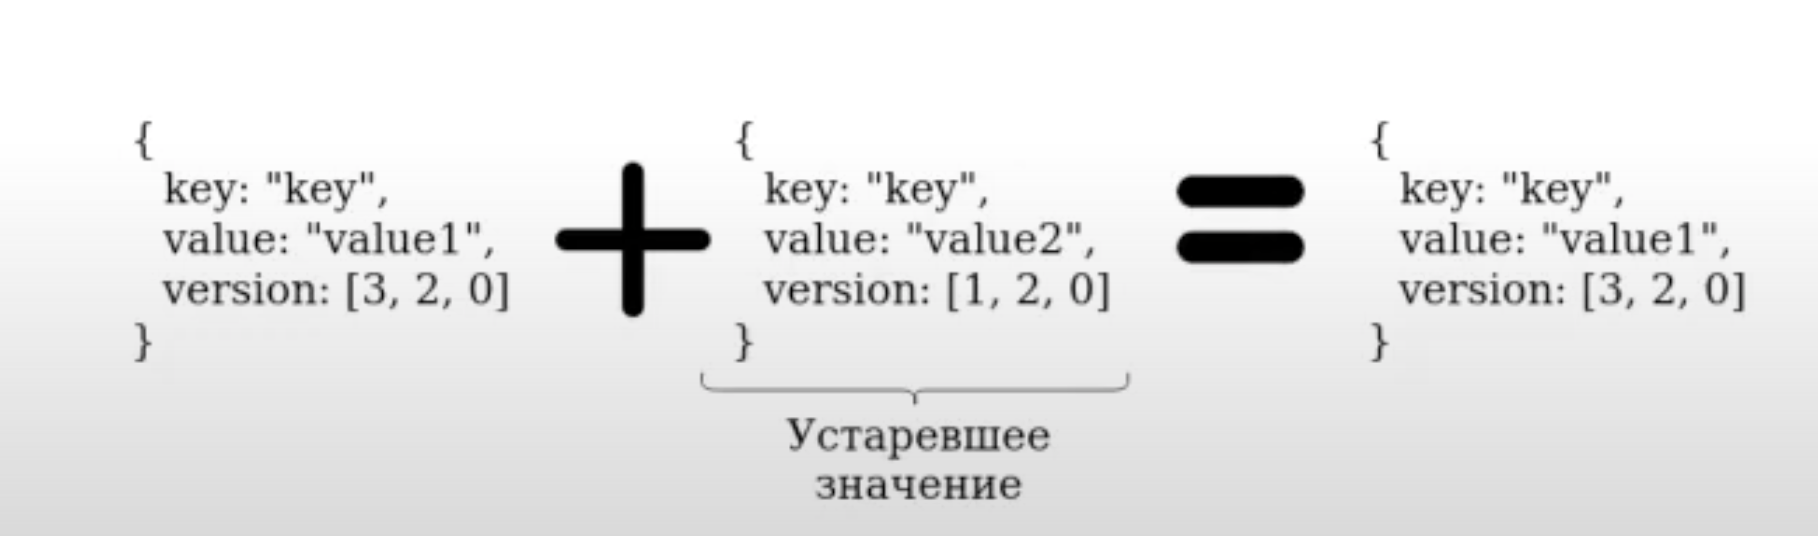
\includegraphics[scale = 0.5]{../assets/2.png}
    \caption{}
\end{figure}
\begin{definition}
  Векторные версии: параллельные обновления
\end{definition}
\begin{itemize}
  \item Параллельность определяется так же, как и в векторных часах.
  \item Мы сами не можем определить, какое значение правильное (так как нет happens-before), тогда сохраним оба значения и пусть приложение само решит, что делать.
  \item Версия получившаяся - покомпонентный максимум из двух несравнимых векторов.
\end{itemize}
\begin{example}
  Приложение может само решать конфликты:\\
  \begin{figure}[h]
      \centering
      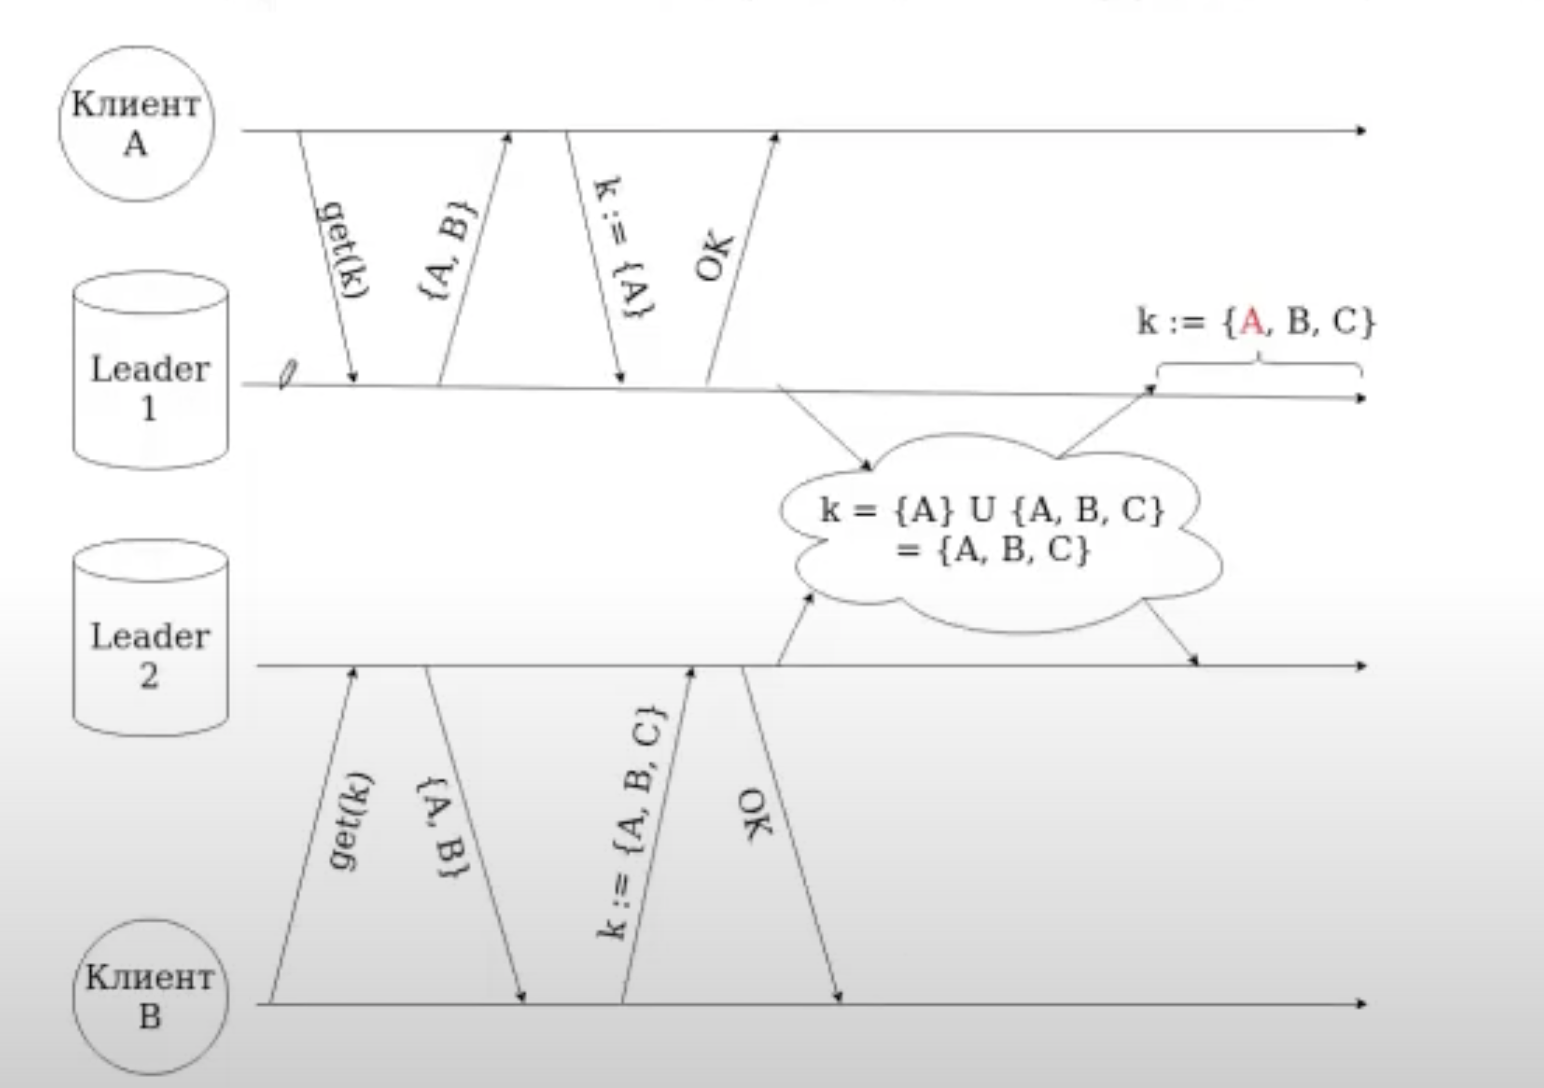
\includegraphics[scale = 0.5]{../assets/4.png}
      \caption{}
  \end{figure}
  \begin{itemize}
    \item Записи $A$ и $B$ параллельны.
    \item Обе операции подтверждаются. Записи происходили одновременно - получаем конфликт.
    \item При решении конфликта - объединении множеств получаем $k = {A} \cup {A, B, C} = {A, B, C}.$
    \item Можем терять только удаление из корзины, но добавление никогда не потеряем.
  \end{itemize}
\end{example}
\begin{definition}
  Разрешение конфликтов при чтении
\end{definition}
\begin{itemize}
  \item Приложение читает данные и понимает, что версии разошлись.
  \item Решает конфликт, получает итоговое значение.
  \item Записывает его в базу.
  \item Увеличивая локальную версию той реплики, куда новая версия будет записана.
  \item Результирующему значению будут предшествовать все конфликтующие записи.
  \item Результирующее значение заменит любое из них.
\end{itemize}
\begin{definition}
  Разрешение конфликтов при чтении на разных узлах
\end{definition}
\begin{itemize}
  \item Конфликт может быть одновременно решен на нескольких узнал, но тогда получаем несравнимые вектора.
  \item Вероятность такого мала, так как конфликт решается при чтении клиентом.
  \item Используем детерменированное разрешение конфликтов.
  \item Как обычно, либо можем сохранить два значение и дать приложению решить конфликт.
  \item Мала вероятность такого конфликта, так как конфликт решается приложением при чтении, то нужно чтобы с двух разных узлов два приложения параллельно прочитали конфликтные значения, узнали что они конфликтные, решили этот конфликт и сделали параллельную запись на два разных узла.
\end{itemize}
\begin{figure}[h]
    \centering
    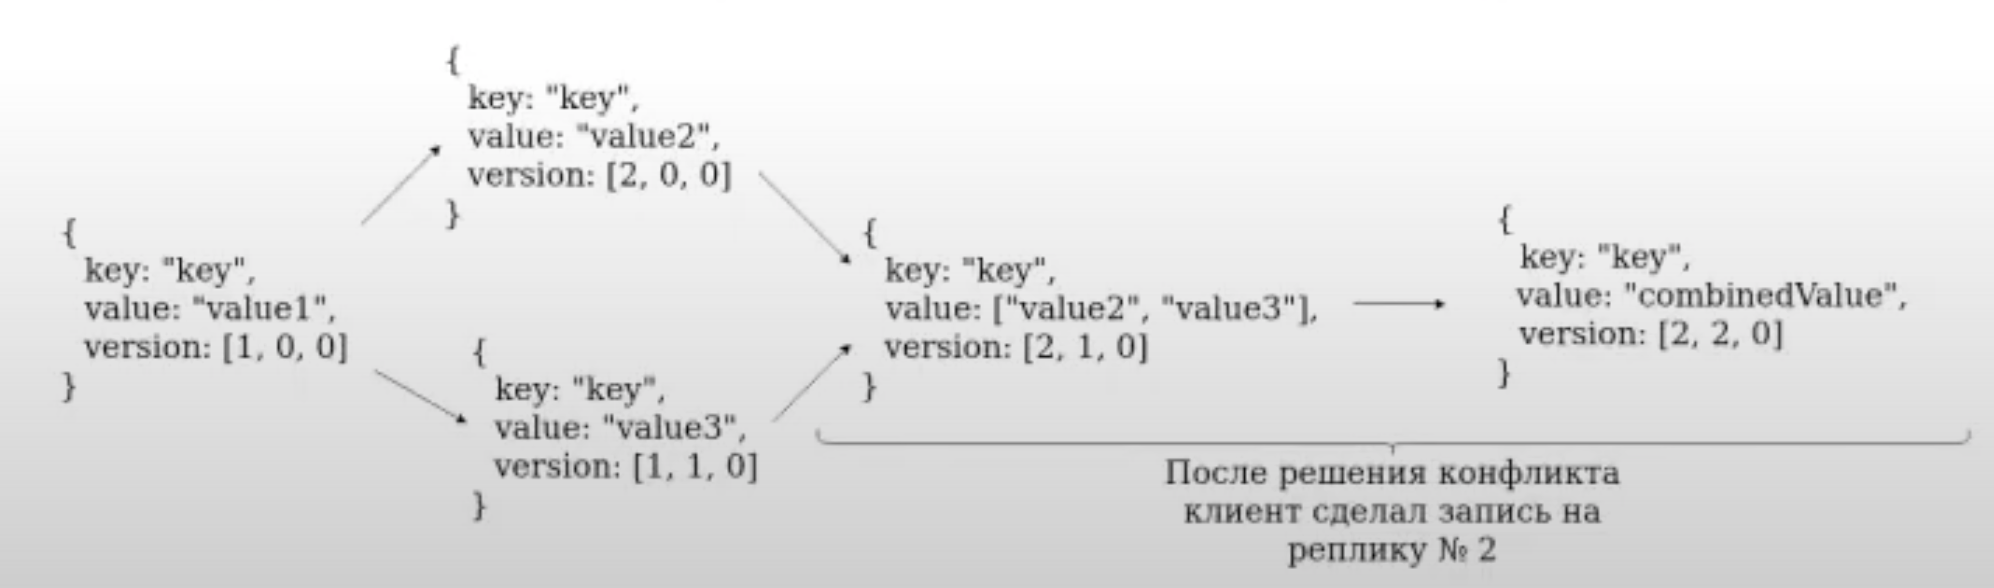
\includegraphics[scale = 0.5]{../assets/5.png}
    \caption{}
\end{figure}
\begin{figure}[h]
    \centering
    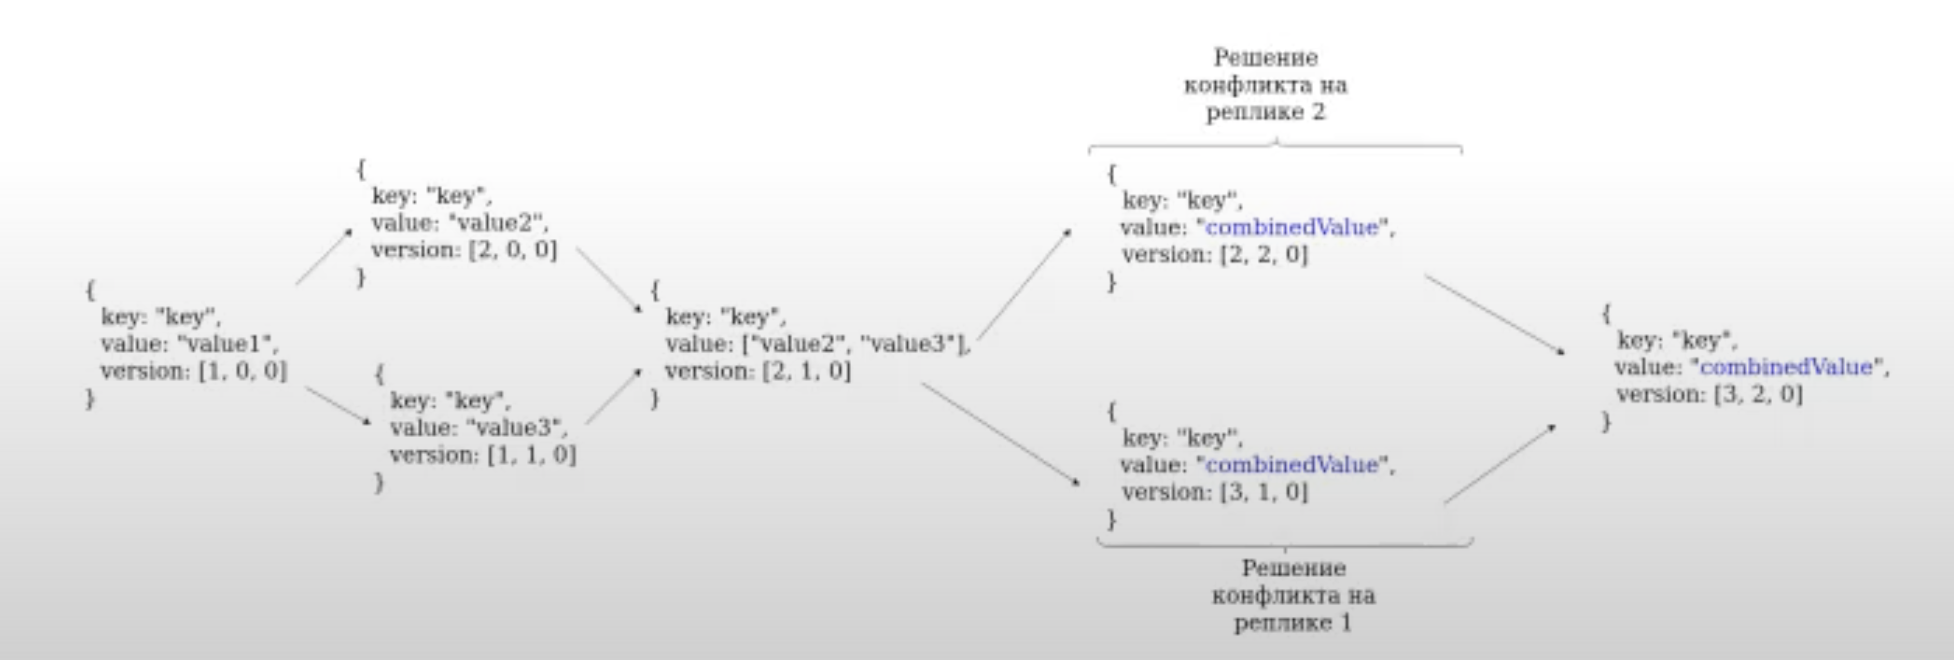
\includegraphics[scale = 0.5]{../assets/6.png}
    \caption{}
\end{figure}
Но и выйти можем по старой схеме - сохранить два конфликтных значения и дать приложению решить конфликт.
\begin{definition}
  Разрешение конфликтов при записи
\end{definition}
\begin{itemize}
  \item Есть конфликты, которые сама реплика может решить при получении конфликтующей версии.
  \item Обычно так решаются очень простые конфликты, которые не требуют вмешательства сложной логики на стороне приложения.
\end{itemize}
\begin{example}
  Параллельная запись в разные поля объекта.\\
  \begin{figure}[h]
      \centering
      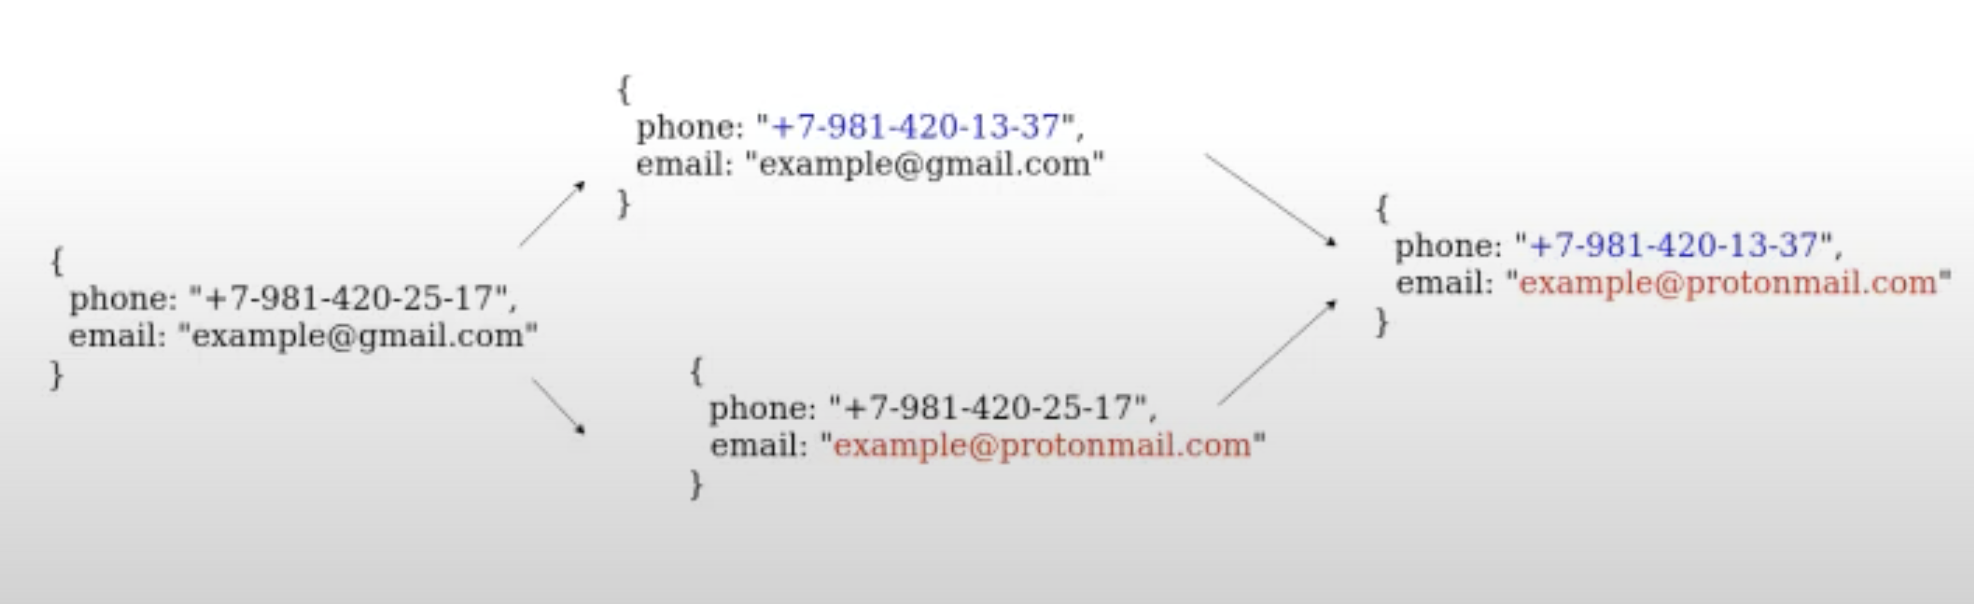
\includegraphics[scale = 0.5]{../assets/7.png}
      \caption{}
  \end{figure}
\end{example}
\begin{definition}
  Невозможность разрешения конфликтов на уровне приложения
\end{definition}
\begin{itemize}
  \item Приложение не может объединить два различных электронных адреса в один корректный, электронный адрес - атомарная сущность, в отличие от корзины с товарами.
  \item У приложения нет возможности узнать как нужно решать конфликт - поскольку нет доступа к реальному миру.
  \item В таком случае можно отдать на разрешение пользователю (так поступает git).
\end{itemize}
\begin{figure}[h]
    \centering
    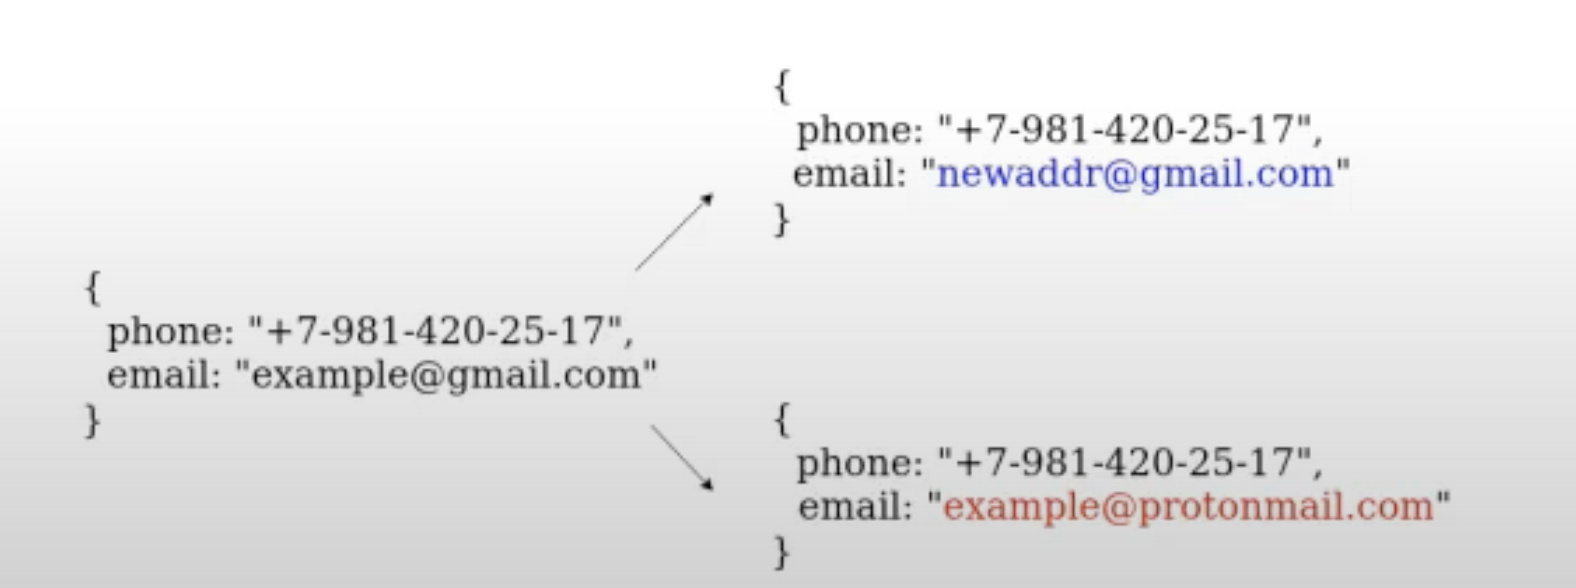
\includegraphics[scale = 0.5]{../assets/8.png}
    \caption{}
\end{figure}
\begin{definition}
  Векторные версии: изменение состава кластера
\end{definition}
\begin{itemize}
  \item Вместо вектора будем хранить отображение.
  \item Ключ - имя узла. Значение - сколько обновлений с этого узла мы видели.
  \item Если же в отображении нет нужного нам ключа - то представим, что он там есть, и значение $0$. Разумно, так как мы не видели ни одного обновления с этого узла.
\end{itemize}
\begin{definition}
  Векторные версии: удаление старых версий
\end{definition}
\begin{itemize}
  \item Мотивация - векторные часы при увеличении количества реплик и не удалении ненужных увеличиваются в размерах.
  \item Хотим удалять старые значения, которые соответствуют выведенным из эксплуатации узлам.
  \item Будем на каждом из узлов помнить, когда мы получали в последний раз сообщение от каждой из реплик.
  \item Из векторных часов будет удалять ключ, который соответствует реплике, от которой дольше всего не получали сообщений, так как с наибольшей вероятностью эта реплика мертвая.
  \item Есть возможность потерять отношение happens-before.
\end{itemize}
\begin{figure}[h]
    \centering
    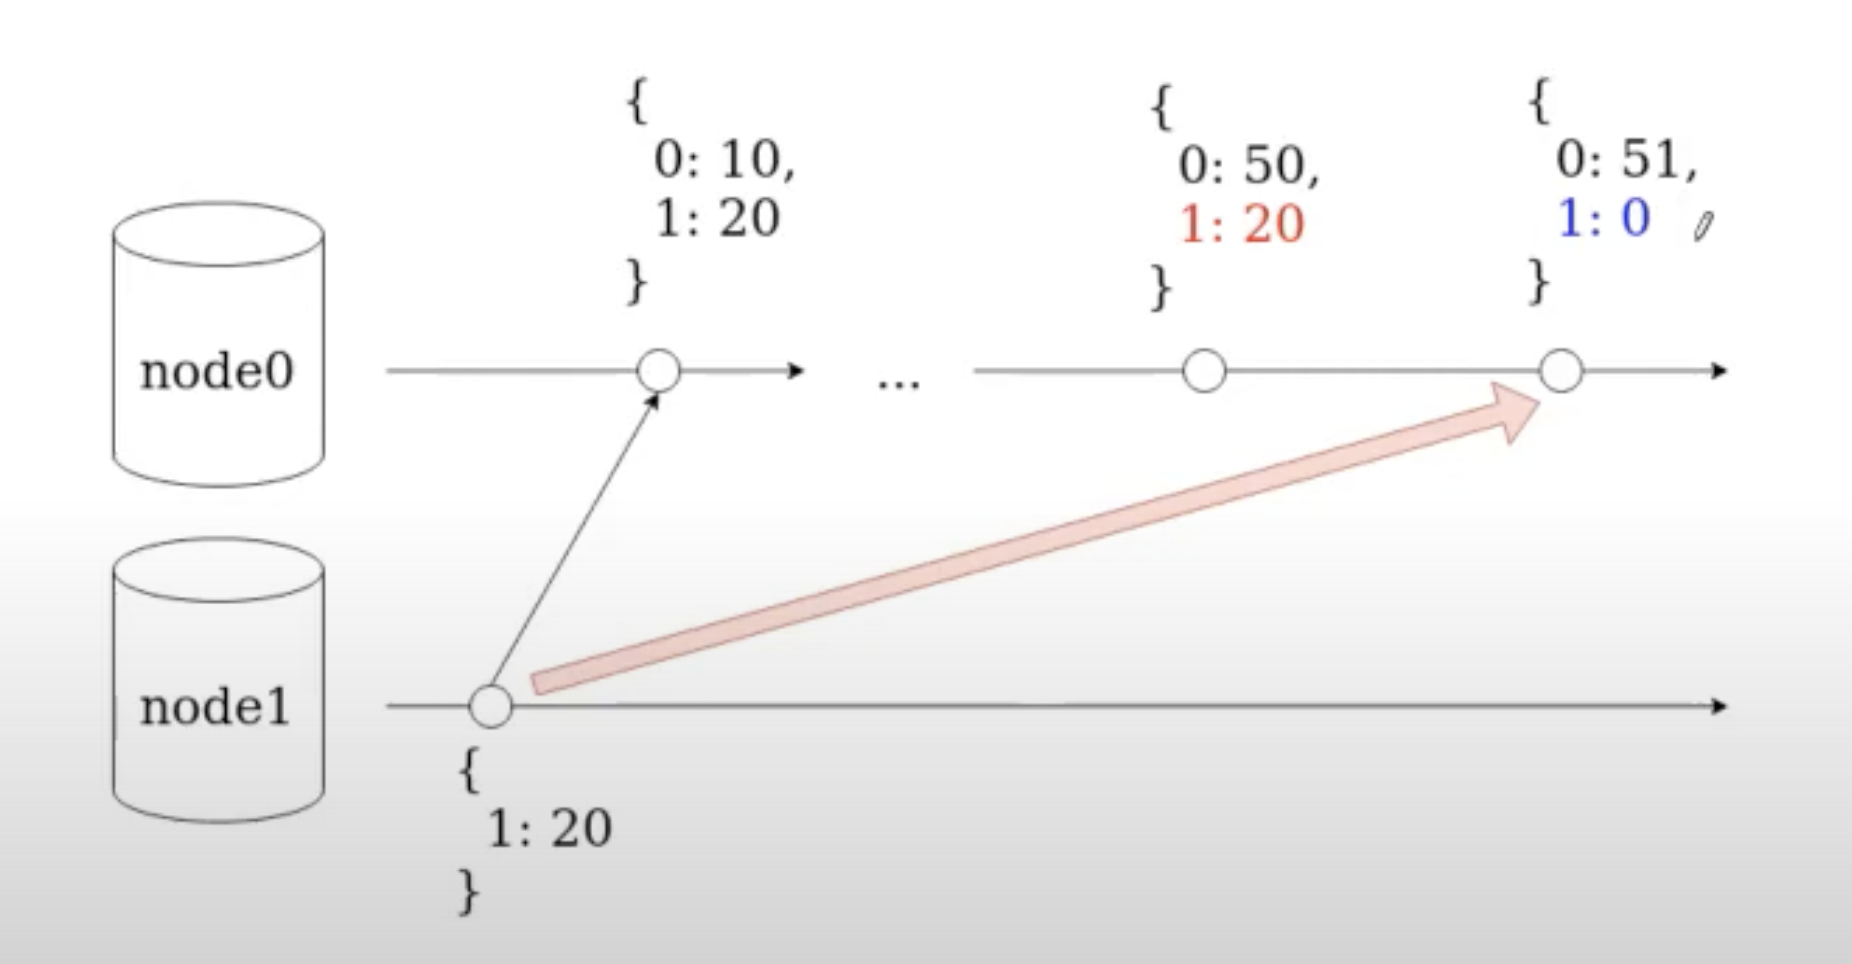
\includegraphics[scale = 0.5]{../assets/9.png}
    \caption{}
\end{figure}
Если у нас есть метод объединения кофликтующих версий - просто объединим эти версии.\\
Вместо удаления старой версии.
